\documentclass{article}

\usepackage[preprint,nonatbib]{neurips_2019}
\usepackage[utf8]{inputenc}
\usepackage[T1]{fontenc}
\usepackage{hyperref}
\usepackage{url}
\usepackage{booktabs}
\usepackage{amsmath,amssymb}
\usepackage{graphicx}
\usepackage{microtype}
\usepackage{enumitem}
\usepackage{xcolor}
\usepackage{float}

\definecolor{navy}{HTML}{1D3557}
\definecolor{tealc}{HTML}{1F8A8C}
\definecolor{coral}{HTML}{C0394D}
\definecolor{slatec}{HTML}{475569}

\hypersetup{
  colorlinks=true,
  linkcolor=navy,
  citecolor=tealc,
  urlcolor=navy
}

\title{Why RL Agents Fail to Use What They Infer in IIGs}

\author{
  Nicholas Erup Larsen \\
  Student ID 2026400695 \\
  IIIS, Tsinghua University \\
  \texttt{nglsls26@mails.tsinghua.edu.cn}
  \And
  Adriaan Van der Berg \\
  Student ID 2026403362 \\
  IIIS, Tsinghua University \\
  \texttt{adla26@mails.tsinghua.edu.cn}
}

\usepackage{pifont}
\newcommand{\Spade}{\ding{171}}
\newcommand{\Club}{\ding{168}}
\newcommand{\Heart}{\textcolor{red!75!black}{\ding{170}}}
\newcommand{\Diam}{\textcolor{red!75!black}{\ding{169}}}
\begin{document}
\raggedbottom

\maketitle
\suppressfloats[t]

\begin{abstract}
Reinforcement learning agents acting under hidden information are often judged by whether that information can be decoded from their internal state, on the assumption that an agent which knows more will act better.
We test this assumption in a multi-agent trading game with a single hidden payoff variable. There, recurrent PPO agents leave almost all of that variable's value unused, and supplying them with an accurate learned belief barely helps.
Using linear probes, agents shown the true hidden state, and interventions that hold the belief fixed while changing only how it reaches the policy, we separate the agent's failure to infer from its failure to act.
The bottleneck is action rather than inference. PPO training weakens what the network encodes, while restructuring the belief-to-policy interface recovers most of the available value both zero-shot and in live training, with only a small gain in probe-measured information.
Probe accuracy alone therefore cannot tell how much of its knowledge an agent can use, and the interface between belief and policy deserves as much attention as the belief itself. Code is available at \url{https://github.com/nicholaseruplarsen/figgie-rl}.

\end{abstract}


\begin{figure}[t]
  \centering
  \begin{minipage}[b]{0.40\textwidth}\centering
    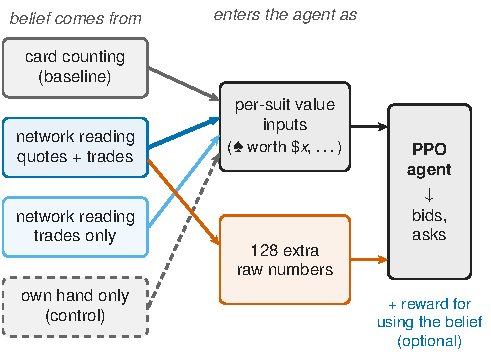
\includegraphics[width=\linewidth]{figs_paper/arms.pdf}
  \end{minipage}\hfill
  \begin{minipage}[b]{0.58\textwidth}\centering
    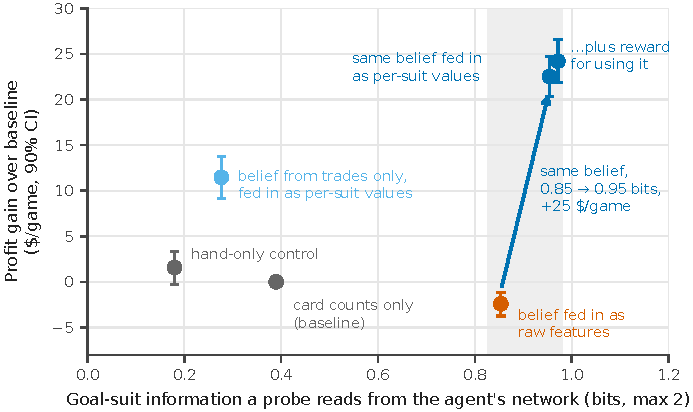
\includegraphics[width=\linewidth]{figs_paper/teaser.pdf}
  \end{minipage}\\[2pt]
  \begin{minipage}[t]{0.40\textwidth}\centering{\small (a) How each agent gets its belief}\end{minipage}\hfill
  \begin{minipage}[t]{0.58\textwidth}\centering{\small (b) What retrained agents know and earn}\end{minipage}
  \caption{How each retrained agent gets its goal-suit belief, and what it knows and earns.}
  \label{fig:teaser}
\end{figure}

\section{Introduction}
\label{sec:intro}

An agent that acts under partial observability has two jobs. It must infer the hidden state from what it sees, and it must turn that inference into good actions. Work on representation learning in RL usually tests only the first job, by training a simple classifier, called a probe, to read the hidden state from the agent's internal memory \cite{alain2016probes,gregor2019belief,mcgrath2022alphazero}. If the probe succeeds, the agent is said to ``know'' the hidden state, and any remaining weakness in its play is blamed on training rather than on knowledge. We test whether probe accuracy is a safe stand-in for what the agent can actually use, and find that it is not (Figure~\ref{fig:teaser}). % √

To investigate this, we study a setting where knowing the hidden state and acting on it can be measured separately. In the four-player trading game Figgie, a single hidden variable decides the payoffs, so we can measure exactly how much that variable is worth, how much of it the agent's network encodes, and how much profit the agent extracts from it. Each of three interventions tests one step of the path from hidden suit to belief to action. We reveal the variable to the agent directly, which shows what perfect knowledge is worth. We give it a belief learned by a separate supervised network, which shows whether a good belief is enough. Finally, we keep that belief fixed and change only how it enters the policy, which shows whether the interface is the bottleneck. % √

In Figgie, 40 cards are dealt from one of 12 equally likely decks, in which one suit has 12 cards, one has 8 and two have 10.
The goal suit is the same-color partner of the 12-card suit (\Spade$\leftrightarrow$\Club, \Heart$\leftrightarrow$\Diam), meaning every player must infer it from their own hand and how others publicly trade, aiming to buy goal cards cheaply before the rest catch on, and before 240 ticks ends the game.
Each goal card pays its holder \$10 at the end, and the rest of the \$200 pot goes to whoever holds the most goal cards. % √
\newpage

Published agents~\cite{figment,figgiebot,cs224r2025figgie} update the goal posterior from their own cards and public order flow with hand-written rules, but none learn that inference from data or tests whether it is used well.
Because the hidden state is tiny, the exact belief is cheap to compute and can be compared with what a network represents.

Knowing is not earning. Each bar pair in Figure~\ref{fig:teaser}b is a PPO agent from one retraining run. The left panel shows how much goal-suit information a probe reads from its network, and the right panel its profit over an agent that sees only card counts (90\% intervals). In the shaded rows the same belief is fed in two ways and the networks hold nearly the same information, yet one agent loses money and the other gains about \$25 per game.

Our contributions thus far are as follows.
\begin{enumerate}[leftmargin=1.4em,itemsep=1pt,topsep=2pt]
  \item We show that recurrent PPO agents leave almost all the value of the hidden information unused, even though a small supervised network can infer it from the same inputs (Sections~\ref{sec:gap} and~\ref{sec:inference}).
  \item We show that the bottleneck is acting on the belief rather than forming it. An accurate belief barely helps, while changing only how the belief enters the policy recovers most of the lost value (Sections~\ref{sec:action} and~\ref{sec:interface}).
  \item We map the limits of this fix, including a collapse against unfamiliar opponents when the agent is rewarded for using its belief (Section~\ref{sec:limits}).
\end{enumerate}

The lesson for RL is that probes overstate usable knowledge, and that the interface between belief and policy matters as much as the quality of the belief (Section~\ref{sec:discussion}).


% =============================================================================
\section{Setup and Methods}
\label{sec:setup}
% =============================================================================

\subsection{Environment}
We use Figgie, a four-player zero-sum card-trading game in which players post and accept prices in one continuous market \cite{disilvio2025figgie,cs224r2025figgie}. We chose it because one hidden variable, the goal suit, decides almost all of the payoff. That lets us measure what an agent knows about the hidden state in bits and what the knowledge is worth in dollars. Each player sees only its own hand and the public quotes and trades over 240 ticks. Nothing in our analysis depends on Figgie beyond this structure.

\subsection{Agents}
Our main agent is a recurrent policy trained with proximal policy optimization (PPO) \cite{schulman2017ppo}. It starts from behaviour cloning, follows the recipe of \cite{cs224r2025figgie}, and uses a GRU as its memory. Besides the market state, its input contains 16 hand-crafted features that describe how much each suit is likely to be worth. By default these come from exact card counting. For every player and suit, card counting tracks the fewest cards that player must hold, given the agent's own hand and every trade so far, and turns these lower bounds into an exact posterior over the 12 possible decks \cite{disilvio2025figgie,cs224r2025figgie}. We call them the agent's per-suit value inputs. Each tick the policy picks one of 257 discrete actions, namely waiting, posting a bid or an ask on a suit at a whole-dollar price from \$1 to \$30 (240 actions), cancelling its own bid or ask on a suit, or buying at the best ask or selling at the best bid on a suit. Actions the game would reject, such as selling a card the agent does not hold, are masked out. We also use two scripted traders, a Bayesian trader and an adaptive market maker, whose actions are a fixed function of a belief about the goal suit. Agents play against one of three tables. The evaluation table seats three scripted traders, a fair-value trader, a Bayesian trader and a market maker. The unseen table seats market makers ported from the open-source Figgie bots figment and Figgie-bot. The third table seats three copies of the PPO agent. During PPO training each of the three opponent seats is filled independently. With probability 30\% it holds a past snapshot of the agent, drawn from the last 16 and weighted toward those the agent beats least often. Otherwise it holds one of five scripted traders chosen uniformly, a random, fair-value, conservative, market-making or Bayesian trader, so each appears 14\% of the time. Figure~\ref{fig:arch} shows the agent and how it is trained.

\begin{figure}[t]
  \centering
  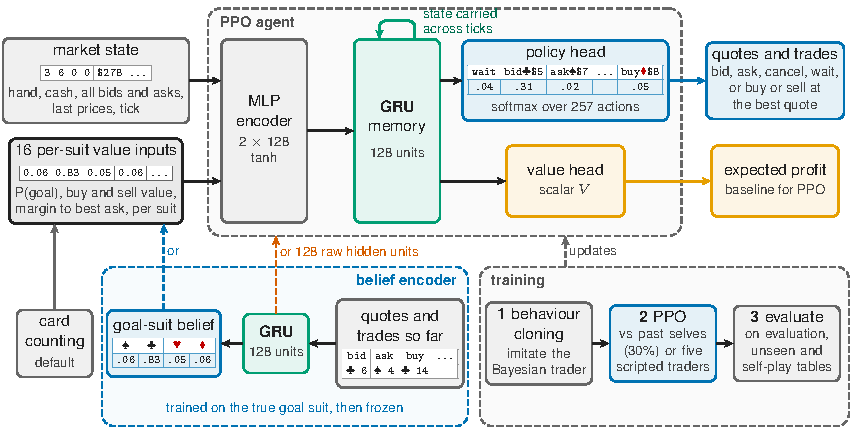
\includegraphics[width=\textwidth]{figs_paper/architecture.pdf}
  \vspace{-8pt}
  \caption{The PPO agent, where its per-suit value inputs come from, and how it is trained.}
  \label{fig:arch}
\end{figure}

\subsection{Measuring what the agent knows}
A linear probe is a simple classifier trained to read the goal suit from a network's hidden state.\footnote{All our probes are linear. We plan to repeat the main measurements with small MLP probes later} We score it on held-out games and report its accuracy or its mutual information with the goal suit in bits. The goal suit takes four equally likely values, so 2 bits means perfect knowledge. A probe can read information that a network merely passes through from its input \cite{hewitt2019control}. We therefore compare every trained network with an untrained copy of the same architecture and with a probe on the raw input. In the retraining study the probe's regularization is tuned by cross-validation, and the probe is checked against copies trained on shuffled labels, which should read nothing. As a known-answer test, we hide a synthetic 1-bit signal in the input and check how much of it the probe recovers.

\subsection{Measuring what the agent does with it}
\label{sec:measure-do}
We give the agent information about the goal suit in four ways and measure the change in profit. The \emph{oracle} reveals the true suit. The second way appends the hidden state of a separately trained supervised network, the \emph{encoder}, to the policy's input as raw features. The third writes the encoder's belief into the existing per-suit value inputs instead. The fourth uses an \emph{opponent-only encoder}, which sees what the other players do but not the agent's own hand, cash and quotes.

To price partial information, we replace the oracle with a noisy signal that carries $I$ bits about the goal suit and is revealed at tick $t$. The signal names one suit, which is the goal suit with probability $\alpha$ and otherwise one of the other three at random. Setting $\alpha$ from $0.25$ to $1$ sweeps $I$ from 0 to 2 bits, so a 1.15-bit signal is right 85\% of the time. The agent's card-counting posterior is updated with the signal by Bayes' rule and fed to it through the per-suit value inputs. We fit
\begin{equation}
  V(I, t) = V_0 \left(\frac{I}{2}\right)^{\gamma} \left(1 - \frac{t}{240}\right)^{\delta},
  \label{eq:voi}
\end{equation}
where $V_0$ is the value of perfect information at the start of the game, $\gamma$ sets how value grows with information, and $\delta$ sets how fast it decays over the game. We chose this form because it is the simplest one that is 0 without information, equals $V_0$ for perfect information at the start, and vanishes at the last of the 240 ticks. One exponent then sets the curvature along each axis. Figure~\ref{fig:voi} in Section~\ref{sec:gap} shows the measurements and the fit.


\subsection{Evaluation}
Every comparison plays both conditions on the same deals, 1,500 to 3,000 per condition, and reports bootstrap 90\% confidence intervals. A \emph{gain} is profit in dollars per game over a matched baseline that differs only in the change being tested. In the \emph{retraining study}, six PPO agents, one per way of feeding in the belief, start from the same weights and train for 400 PPO updates on three seeds, unlike the frozen agents elsewhere. Each main comparison was pre-registered with a 90\% prediction interval and a placebo control before it ran.

% =============================================================================
\section{Results so far}
\label{sec:results}
% =============================================================================

\subsection{RL agents leave the hidden information unused}
\label{sec:gap}

\begin{figure}[H]
  \centering
  \begin{minipage}[b]{0.49\textwidth}\centering
    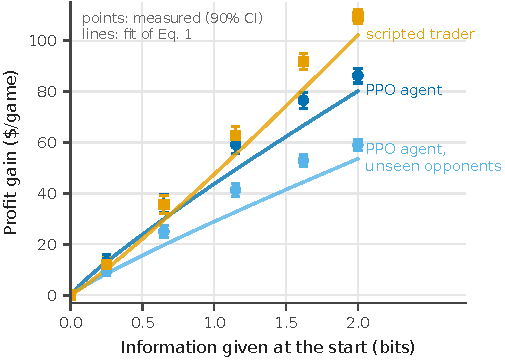
\includegraphics[width=\linewidth]{figs_paper/voi.pdf}\\[-2pt]
    {\small (a) three agents, signal at tick 0}
  \end{minipage}\hfill
  \begin{minipage}[b]{0.49\textwidth}\centering
    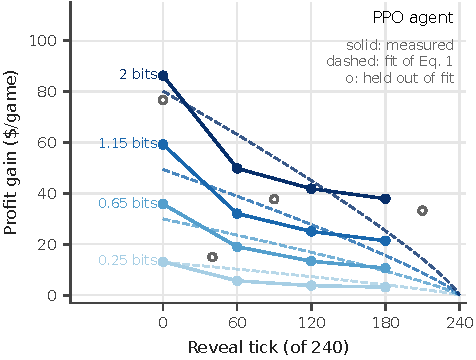
\includegraphics[width=\linewidth]{figs_paper/voi_tick.pdf}\\[-2pt]
    {\small (b) PPO agent, signal at tick $t$}
  \end{minipage}
  \caption{Value of a goal-suit signal against its information content (a) and its reveal tick (b).}
  \label{fig:voi}
\end{figure}

How much is the goal suit worth to a trained PPO agent? A great deal. Revealing it at the start of the game adds about \$86 per game (Figure~\ref{fig:voi}a). Panel (a) gives the agent the noisy signal of Section~\ref{sec:measure-do} at tick 0 and varies its information from nothing to the full 2 bits. Points are measured gains for the frozen PPO agent and a scripted trader (90\% CIs, 1,500 paired deals each), and lines are fits of Eq.~\ref{eq:voi}. Value grows roughly in proportion to information, so even a fraction of a bit is worth a lot. Against unseen opponents the PPO curve keeps its shape but sits lower.

Panel (b) shows the PPO agent alone and delays the hint instead. Each solid line holds the information fixed and moves the reveal from tick 0 to tick 180. Most of the value is lost in the first 60 ticks, after which it levels off. A full 2-bit hint is worth about \$86 at the start, \$50 at tick 60 and \$38 at tick 180. The fit of Eq.~\ref{eq:voi} (dashed) misses this front-loaded decay and predicts about \$63 at tick 60, so it describes the information axis well but understates how quickly information goes stale. Open circles were held out of the fit.

This ceiling is what makes the trained agent's behaviour striking. The agent sees the order flow that carries this information on every tick. Yet, as the next two sections show, almost none of it appears in its profit or in its hidden state.


\subsection{The failure is not inference}
\label{sec:inference}

Is the goal suit hard to infer from what the agent sees? No. A small supervised network, trained to predict the goal suit from the same input sequence, reaches far higher probe accuracy than a probe on the current input alone (Figure~\ref{fig:activations}). The figure tracks a linear probe at every tick over 300 games (90\% bootstrap bands). In a single example game only the supervised network commits to the true suit (Appendix Figure~\ref{fig:example}), and the raw activations show no pattern readable by eye, which is why we use probes (Appendix Figure~\ref{fig:heatmaps}). The information is in the history, and it can be learned.

PPO does not learn it in 33M environment steps (2,000 PPO updates, 128,000 games), and training makes things worse (Figure~\ref{fig:activations}). A probe reads the goal suit less well from the PPO agent's trained network than from its raw input or from an untrained copy of the same network. The same holds for every architecture we tested, a GRU, a minGRU \cite{feng2024mingru}, a Transformer and a network with no memory (Appendix Figure~\ref{fig:mirage}). That comparison uses 3,000 games and two seeds per architecture, so its input baseline differs from Figure~\ref{fig:activations}. Every core knows less after PPO training. We call this the \emph{probe mirage}. A probe on a trained agent seems to show knowledge, but most of what it reads is already present in a random network, and RL training removes some of it. Once probe width is matched, the network without memory does as well as the recurrent ones, so recurrent memory adds nothing that the probe can find.

\begin{figure}[t]
  \centering
  \begin{minipage}[t]{0.49\textwidth}\centering
    \vspace{0pt}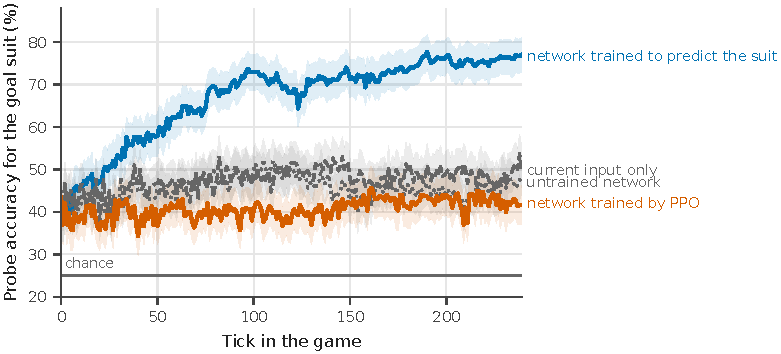
\includegraphics[height=5cm]{figs_paper/probe.pdf}
  \end{minipage}\hfill
  \begin{minipage}[t]{0.49\textwidth}\centering
    \vspace{0pt}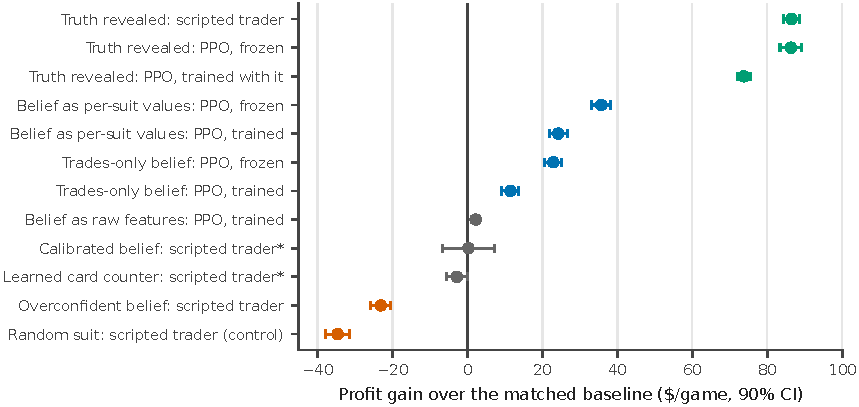
\includegraphics[height=5cm]{figs_paper/payoff_ladder.pdf}
  \end{minipage}\\
  \begin{minipage}[t]{0.49\textwidth}
    \caption{Mean goal-suit probe accuracy by tick over 300 games.}
    \label{fig:activations}
  \end{minipage}\hfill
  \begin{minipage}[t]{0.49\textwidth}
    \caption{Profit gain for each way of giving the agent the goal suit.}
    \label{fig:ladder}
  \end{minipage}
\end{figure}

\subsection{The failure is in action}
\label{sec:action}

Handing the agent a good belief barely closes the gap. We appended the encoder's hidden state to the PPO agent's input as raw features and retrained it. A probe then reads the goal suit from the policy much better, but profit hardly moves and captures about 3\% of the oracle's value (Figure~\ref{fig:ladder}). The truth is worth a lot, a raw belief almost nothing. In the figure, ``frozen'' agents were not retrained, ``trained'' agents were trained with the change, rows marked * are exploratory pilots, and bars show 90\% CIs. The agent knows much more by the probe's measure and uses almost none of it.

A belief can even cost money. A scripted trader acts as a fixed function of its belief, which takes RL out of the question. Given the true suit, it gains about as much as the oracle gives the PPO agent. Given the encoder's belief, it loses money compared with exact card counting (Figure~\ref{fig:ladder}). Overconfident beliefs lose money. The encoder was trained, as a standard sequence classifier, only on its prediction at the end of each game, so it was confidently wrong early on, and a change of opponents lowered its accuracy further. In exploratory pilots, temperature scaling \cite{guo2017calibration}, a one-parameter correction for overconfidence, recovers most of the loss. It cuts the calibration error at the last tick from 0.39 to 0.14 for the original encoder and from 0.44 to 0.17 for one retrained at every tick on a mix of opponents, against 0.10 for exact card counting, and the retrained encoder then beats the card counter by \$8 per game. A calibrated neural copy of the card counter still loses a little, which suggests a small cost for any learned belief. A belief that is right on average can be worth less than none if its confidence is wrong, and the actor cannot tell.

\subsection{Changing only the interface recovers most of the value}
\label{sec:interface}

Changing only the step from belief to action helps, even without retraining the agent. We left the trading agent exactly as it was and changed only what it is told about the goal suit and where in its input that goes, one thing at a time (Figure~\ref{fig:chasm}). Writing the belief into the per-suit value inputs, instead of appending raw features, helps. An encoder trained, as is standard, only to classify the finished game gives overconfident beliefs mid-game, so supervising it at every tick helps more, and training it against the same opponents as at evaluation helps again. The last change hides the agent's own hand, cash and quotes from the encoder. Together the four changes recover most of the value that the same information would give if it were handed over directly. In Figure~\ref{fig:chasm} the first bar is the PPO agent retrained with the belief as raw features, the others use the frozen agent over 2,000 paired deals, and the dashed line is the value of the same information handed over directly.

The last change matters because of a feedback loop that traders call reflexivity, a case of what machine learning calls performative prediction \cite{perdomo2020performative}. An encoder trained on one agent's games learns to treat that agent's own cards and quotes as evidence about the goal suit. When another agent produces those signals, or the same agent starts acting on the belief, they no longer mean the same thing, and the belief corrupts itself. An encoder that sees only the opponents avoids the loop. The rescue holds for three different traders and when a different agent records the training games (Appendix Figure~\ref{fig:trap}). Hiding the agent's own actions rescues the belief. That figure compares an encoder that sees everything (open) with one that sees only the opponents (filled), for encoders recorded on PPO games and on Bayesian-trader games. An encoder that sees only completed trades, with no quotes, keeps most of the gain, so the effect does not come from scripted opponents revealing their hands through their quotes.

\begin{figure}[t]
  \centering
  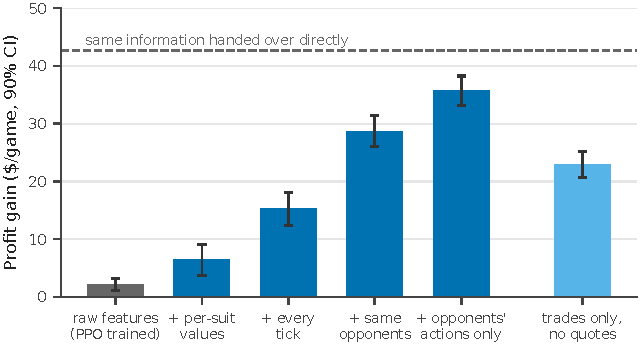
\includegraphics[width=0.8\textwidth]{figs_paper/interface.pdf}
  \caption{Profit gain as four interface changes are added in turn.}
  \label{fig:chasm}
\end{figure}

Within our budget, PPO does not learn by itself to turn a belief into prices, so feeding the belief through the per-suit value inputs is still needed. We trained six PPO agents from the same starting point (Figure~\ref{fig:teaser}, Table~\ref{tab:e2b}). The agent given the opponent-only encoder as raw features ends slightly below the card-count baseline, although a probe finds a lot of goal-suit information in its network. The agent given the same encoder through its per-suit value inputs more than doubles the baseline's profit, with only slightly more probe-measured information. A placebo that fills the value inputs from the agent's own hand stays near the baseline. After 400 updates, PPO had still not learned the step from a belief to prices that the per-suit inputs provide for free.

\subsection{Limits}
\label{sec:limits}

The fix does not hold against different opponents. The encoder was trained against scripted opponents whose trading gives away their hands. Against three copies of the PPO agent, which give away much less, the agents with the per-suit belief fall below the card-count agent, and the frozen agents with an encoder plugged in fall further (Figure~\ref{fig:selfplay}). Gains against familiar opponents do not transfer. In the figure, dots are agents trained with each input, open diamonds are the frozen agent with an encoder plugged in, and the blue arrow shows what adding a reward for using the belief does to the per-suit agent. Rewarding the agent for acting on its belief, through potential-based reward shaping \cite{ng1999shaping}, adds a little against familiar opponents and makes the drop against PPO opponents much worse. The belief helps only while the opponents behave like the ones it was trained on.

\begin{figure}[t]
  \centering
  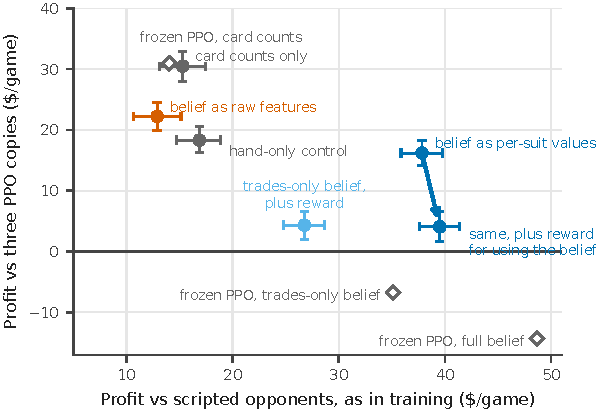
\includegraphics[width=0.6\textwidth]{figs_paper/selfplay.pdf}
  \caption{Profit against scripted opponents and against PPO opponents.}
  \label{fig:selfplay}
\end{figure}

One causal test failed. In an earlier study we added an auxiliary loss that trained the PPO network to predict the goal suit, to test whether supervising the representation helps. Its placebo, the same loss with shuffled labels, changed profit by more than the pre-set tolerance on all three seeds. We treat that test as invalid rather than as a null result and make no claim about auxiliary losses. The placebo's effect may come from the extra loss acting as a regulariser, which we did not test.

The scope is narrow. All results come from one game with one discrete hidden variable. The retraining study uses three seeds and 400 updates per agent, fewer than our pilot found necessary for stable rankings, so the order of close agents could change with longer training. Its known-answer probe check fell just short of its pre-set bar, so the probe values in Figure~\ref{fig:teaser} are indicative and probably read low. The probe was also run on one seed only. The zero-shot interface study failed its placebo gates as well, so both studies give evidence rather than proof. We did not test a simpler rival to the per-suit inputs, a learned linear map from the encoder's output to the same inputs. The predictions for the retraining study were recorded after its code was frozen and before launch, its pilot and test games do not overlap, and all three seeds exist.

% =============================================================================
\section{Discussion}
\label{sec:discussion}
% =============================================================================

\subsection{Probes overstate usable knowledge}
Probing shows what a network contains, not what the agent can use. Linear probes are a standard way to ask what a network represents \cite{alain2016probes,belinkov2022probing}, and control tasks were introduced because a probe can find structure that the model does not use \cite{hewitt2019control}. Our results add two cautions for RL. Untrained recurrent networks already pass much of the input through, so a trained agent should be compared with its untrained copy, and in our case RL training lowered what a probe could read. More importantly, what a probe reads and what the agent uses come apart. Two retrained agents with nearly the same probe-measured information differ widely in profit, and appending a belief raises probe accuracy with almost no change in reward.

\subsection{The interface matters as much as the representation}
Belief-state methods for partially observable problems \cite{kaelbling1998pomdp} and their deep variants \cite{hausknecht2015drqn,igl2018dvrl} aim to make the agent's state a good belief. Auxiliary losses \cite{jaderberg2017unreal} push the representation toward useful features. Both target the representation. In our setting the representation was not the binding constraint. What mattered was whether the belief arrived in a form the policy could turn into actions, and whether it depended on the agent's own behaviour. A calibrated belief that depends only on the opponents, written into features the policy already acts on, was worth far more than a richer latent. Work on belief-state RL could report the step from belief to action separately, for example with the oracle and fixed-belief interventions we use here.

\subsection{Future work}
Before the final report, we intend to train longer with tuned hyperparameters, at 0.4B-1B steps per agent, to see whether PPO learns the step from belief to prices by itself. We will also test the simpler rival, a learned linear map from the encoder to the per-suit inputs, and rerun the retraining probe and the recall test on all seeds with valid placebos. Beyond that, three directions follow from our results. The per-suit inputs work because we hand-coded what each suit is worth. A learned module that treats every suit alike (suit-equivariant), without that formula, would show whether the gain carries over to games where no such formula exists. The value of information falls steeply over the game, so agents might learn to quote early just to draw informative fills. Training the belief and the opponents together in a co-evolving population would show whether opponents learn to hide their hands, and what the belief is worth then. Finally, we plan to test whether the probe mirage and the reflexivity loop appear in other games with hidden state, from rock--paper--scissors against biased opponents to Kuhn and Leduc poker, phantom tic-tac-toe, dark hex and maybe the fog-of-war strategy game generals.io.


% =============================================================================
\small
\newcommand{\reftitle}[2]{\href{#1}{\color{black}#2}}
\begin{thebibliography}{20}\setlength{\itemsep}{1pt}\setlength{\parsep}{0pt}

\bibitem{alain2016probes}
G.~Alain and Y.~Bengio.
\newblock \reftitle{https://arxiv.org/abs/1610.01644}{Understanding intermediate layers using linear classifier probes}.
\newblock \emph{arXiv preprint arXiv:1610.01644}, 2016.

\bibitem{belinkov2022probing}
Y.~Belinkov.
\newblock \reftitle{https://doi.org/10.1162/coli_a_00422}{Probing classifiers: Promises, shortcomings, and advances}.
\newblock \emph{Computational Linguistics}, 48(1):207--219, 2022.

\bibitem{cs224r2025figgie}
D.~Yang.
\newblock \reftitle{https://cs224r.stanford.edu/projects/pdfs/Daniel\%20Li\%20Yang\%20submission_416100137/CS224R_Project_Report-5.pdf}{Reinforcement learning for Figgie: Learning negotiation as a first-class skill}.
\newblock Stanford CS224R project report, 2026.

\bibitem{disilvio2025figgie}
S.~DiSilvio, Y.~Luo, and A.~Ozerov.
\newblock \reftitle{https://arxiv.org/abs/2110.00879}{Traders in a strange land: Agent-based discrete-event market simulation of the Figgie card game}.
\newblock \emph{arXiv preprint arXiv:2110.00879}, 2021.

\bibitem{feng2024mingru}
L.~Feng, F.~Tung, M.~O. Ahmed, Y.~Bengio, and H.~Hajimirsadeghi.
\newblock \reftitle{https://arxiv.org/abs/2410.01201}{Were RNNs all we needed?
\newblock \emph{arXiv preprint arXiv:2410.01201}, 2024}.

\bibitem{gregor2019belief}
K.~Gregor, D.~Jimenez Rezende, F.~Besse, Y.~Wu, H.~Merzic, and A.~van~den Oord.
\newblock \reftitle{https://arxiv.org/abs/1906.09237}{Shaping belief states with generative environment models for RL}.
\newblock In \emph{NeurIPS}, 2019.

\bibitem{figment} mneha05.
\newblock figment: a self-play market-making arena for Figgie-style card markets.
\newblock \url{https://github.com/mneha05/figment}.

\bibitem{figgiebot} revilo-25.
\newblock Figgie-bot.
\newblock \url{https://github.com/revilo-25/Figgie-bot}.

\bibitem{perdomo2020performative}
J.~C. Perdomo, T.~Zrnic, C.~Mendler-D\"unner, and M.~Hardt.
\newblock \reftitle{https://arxiv.org/abs/2002.06673}{Performative prediction}.
\newblock In {\em ICML}, 2020.

\bibitem{guo2017calibration}
C.~Guo, G.~Pleiss, Y.~Sun, and K.~Q. Weinberger.
\newblock \reftitle{https://arxiv.org/abs/1706.04599}{On calibration of modern neural networks}.
\newblock In \emph{ICML}, pages 1321--1330, 2017.

\bibitem{hausknecht2015drqn}
M.~Hausknecht and P.~Stone.
\newblock \reftitle{https://arxiv.org/abs/1507.06527}{Deep recurrent Q-learning for partially observable MDPs}.
\newblock In \emph{AAAI Fall Symposium}, 2015.

\bibitem{hewitt2019control}
J.~Hewitt and P.~Liang.
\newblock \reftitle{https://doi.org/10.18653/v1/D19-1275}{Designing and interpreting probes with control tasks}.
\newblock In \emph{EMNLP-IJCNLP}, pages 2733--2743, 2019.

\bibitem{igl2018dvrl}
M.~Igl, L.~Zintgraf, T.~A. Le, F.~Wood, and S.~Whiteson.
\newblock \reftitle{https://arxiv.org/abs/1806.02426}{Deep variational reinforcement learning for POMDPs}.
\newblock In \emph{ICML}, pages 2117--2126, 2018.

\bibitem{jaderberg2017unreal}
M.~Jaderberg, V.~Mnih, W.~M. Czarnecki, T.~Schaul, J.~Z. Leibo, D.~Silver, and K.~Kavukcuoglu.
\newblock \reftitle{https://arxiv.org/abs/1611.05397}{Reinforcement learning with unsupervised auxiliary tasks}.
\newblock In \emph{ICLR}, 2017.

\bibitem{kaelbling1998pomdp}
L.~P. Kaelbling, M.~L. Littman, and A.~R. Cassandra.
\newblock \reftitle{https://doi.org/10.1016/S0004-3702(98)00023-X}{Planning and acting in partially observable stochastic domains}.
\newblock \emph{Artificial Intelligence}, 101(1--2):99--134, 1998.

\bibitem{mcgrath2022alphazero}
T.~McGrath, A.~Kapishnikov, N.~Toma\v{s}ev, A.~Pearce, M.~Wattenberg, D.~Hassabis, B.~Kim, U.~Paquet, and V.~Kramnik.
\newblock \reftitle{https://doi.org/10.1073/pnas.2206625119}{Acquisition of chess knowledge in AlphaZero}.
\newblock \emph{PNAS}, 119(47):e2206625119, 2022.

\bibitem{ng1999shaping}
A.~Y. Ng, D.~Harada, and S.~Russell.
\newblock \reftitle{https://people.eecs.berkeley.edu/~russell/papers/icml99-shaping.pdf}{Policy invariance under reward transformations: Theory and application to reward shaping}.
\newblock In \emph{ICML}, pages 278--287, 1999.

\bibitem{schulman2017ppo}
J.~Schulman, F.~Wolski, P.~Dhariwal, A.~Radford, and O.~Klimov.
\newblock \reftitle{https://arxiv.org/abs/1707.06347}{Proximal policy optimization algorithms}.
\newblock \emph{arXiv preprint arXiv:1707.06347}, 2017.

\bibitem{wijmans2023maps}
E.~Wijmans, M.~Savva, I.~Essa, S.~Lee, A.~S. Morcos, and D.~Batra.
\newblock \reftitle{https://arxiv.org/abs/2301.13261}{Emergence of maps in the memories of blind navigation agents}.
\newblock In \emph{ICLR}, 2023.

\end{thebibliography}

% =============================================================================
\clearpage
\appendix
\normalsize

\section{Retraining study results}
\label{app:e2b}

\begin{table}[H]
  \centering
  \caption{Profit per game of the retrained agents and of frozen references, against scripted (held-in and held-out) and PPO opponents.}
  \label{tab:e2b}
  \small
  \begin{tabular}{@{}lrrrrr@{}}
    \toprule
    & \multicolumn{4}{c}{Profit vs.\ opponents (\$/game, $\pm$ 90\% CI)} & \\
    \cmidrule(lr){2-5}
    Agent & Scripted & Held-out & PPO & Each other & Probe (bits) \\
    \midrule
    \multicolumn{6}{@{}l}{\textit{Retrained for 400 updates, 3 seeds}} \\
    Card counts & $+15.3 \pm 2.2$ & $-1.5 \pm 1.6$ & \underline{$+30.5 \pm 2.5$} & \underline{$+1.4 \pm 1.8$} & $0.390$ \\
    Encoder, raw features & $+12.9 \pm 2.2$ & $-0.6 \pm 1.6$ & $+22.2 \pm 2.3$ & $\mathbf{+3.4 \pm 1.7}$ & $0.854$ \\
    Encoder, per-suit inputs & $+37.9 \pm 2.0$ & $-1.7 \pm 1.6$ & $+16.2 \pm 2.1$ & --- & \underline{$0.954$} \\
    \quad + reward for using belief & \underline{$+39.5 \pm 1.9$} & $-5.1 \pm 1.6$ & $+4.1 \pm 2.5$ & $-3.8 \pm 1.6$ & $\mathbf{0.972}$ \\
    Trades-only encoder + reward & $+26.8 \pm 1.9$ & $-6.7 \pm 1.5$ & $+4.3 \pm 2.4$ & $-1.1 \pm 1.6$ & $0.276$ \\
    Placebo (own hand) & $+16.9 \pm 2.1$ & \underline{$0.0 \pm 1.6$} & $+18.3 \pm 2.1$ & --- & $0.180$ \\
    \midrule
    \multicolumn{6}{@{}l}{\textit{Frozen agent, no retraining}} \\
    Card counts & $+14.1 \pm 2.2$ & $\mathbf{+0.7 \pm 1.6}$ & $\mathbf{+31.0 \pm 2.5}$ & --- & --- \\
    Quotes + trades encoder & $\mathbf{+48.7 \pm 1.6}$ & $-7.6 \pm 1.9$ & $-14.3 \pm 2.5$ & --- & --- \\
    Trades-only encoder & $+35.1 \pm 1.7$ & $-5.3 \pm 1.5$ & $-6.7 \pm 2.6$ & --- & --- \\
    \bottomrule
  \end{tabular}
\end{table}
Each profit is over 3,000 paired deals. Bold marks the best value in each column and underline the second best. ``Each other'' plays the four retrained agents in one game. The probe column is the cross-validated goal-suit information at the last tick, and its shuffled-label null is below 0.13 bits for every agent.

\section{Additional figures}
\label{app:figs}


\begin{figure}[H]
  \centering
  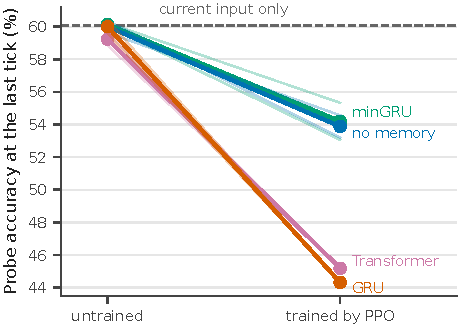
\includegraphics[width=0.5\textwidth]{figs_paper/mirage.pdf}
  \caption{Last-tick probe accuracy before and after PPO training, by architecture.}
  \label{fig:mirage}
\end{figure}

\begin{figure}[H]
  \centering
  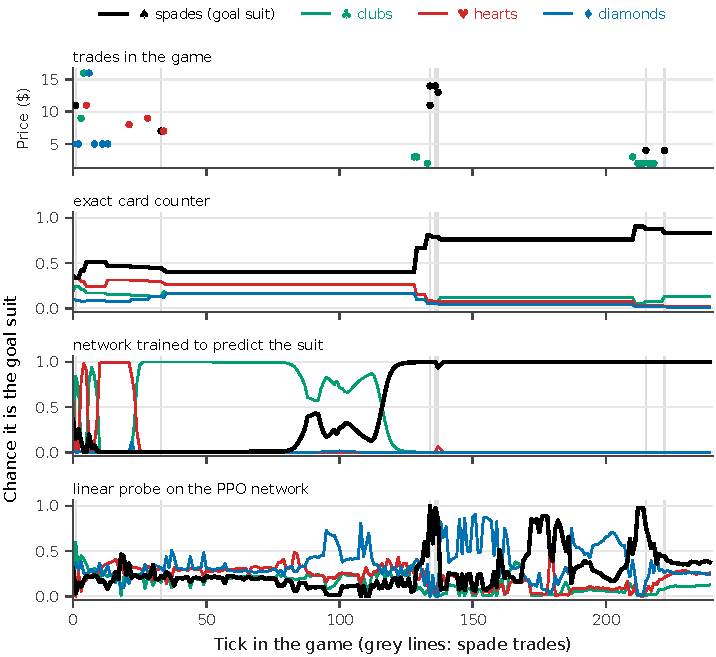
\includegraphics[width=0.9\textwidth]{figs_paper/example_game.pdf}
  \caption{Belief in each suit over one example game (goal suit \Spade).}
  \label{fig:example}
\end{figure}

\begin{figure}[H]
  \centering
  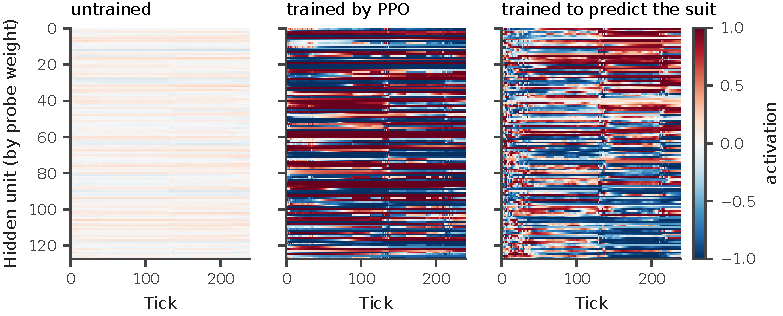
\includegraphics[width=0.9\textwidth]{figs_paper/activations_heatmaps.pdf}
  \caption{Hidden activations of three networks on the example game. Hopefully this will show a useful pattern in the future}
  \label{fig:heatmaps}
\end{figure}

\begin{figure}[H]
  \centering
  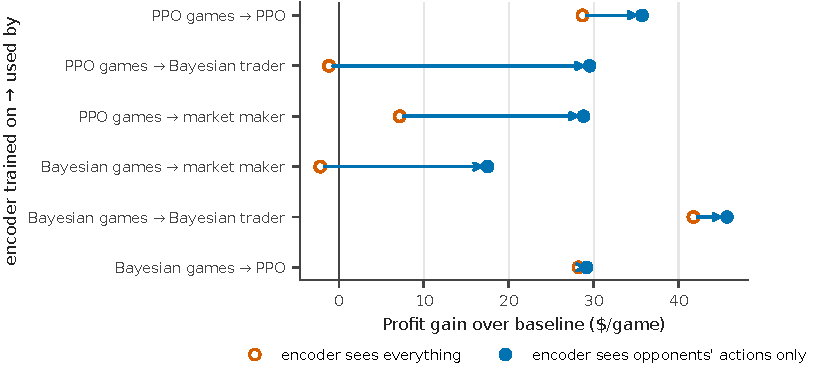
\includegraphics[width=0.85\textwidth]{figs_paper/trap.pdf}
  \caption{Trader gain with a full-view and an opponent-only encoder.}
  \label{fig:trap}
\end{figure}

\end{document}
